% ============================================================
% RESULTS SECTION
% ============================================================

\section{Results}\label{sec:results}

We present the evaluation results for all policies across 500 episodes each, focusing on overall performance, SOFA-stratified analysis, and most importantly, the LEG interpretability comparison that reveals dramatic differences in feature importance patterns across algorithms.

% ============================================================
\subsection{Overall Performance Comparison}\label{sec:results:overall}

Table \ref{tab:overall-performance} and Figure \ref{fig:algorithm-comparison} show results for 8 policies. DDQN-Attention achieves highest survival (95.4\%), with all methods in narrow range (94.0--95.4\%). Online RL achieves marginally higher rates than offline (95.4\%, 94.8\%, 94.2\% vs. 94.2\%, 94.0\%, 94.0\%).

The high baseline survival ($\sim$94--95\%) likely reflects the simulator's forgiving outcome model, underscoring limitations of simulator-only evaluation. Average returns range from 13.20 to 13.62, with high variance from sparse rewards. Online RL's modest gain (1.2-1.4 points) requires 1M training timesteps—infeasible clinically. Offline methods achieve comparable survival (94.0--94.2\%) from pre-collected data only, motivating our focus on interpretability (Section~\ref{sec:results:leg}).

\begin{table}[htbp]
\centering
\caption{Overall performance (500 episodes). Survival rates: 94.0--95.4\%, with DDQN-Attention highest (95.4\%). Online RL marginally outperforms offline but requires environment interaction during training.}
\label{tab:overall-performance}
\begin{tabular}{lcccc}
\toprule
\textbf{Model} & \textbf{Survival (\%)} & \textbf{Avg Return} & \textbf{Avg Length} & \textbf{Paradigm} \\
\midrule
\multicolumn{5}{l}{\textit{Baselines}} \\
Random          & 95.0               & 13.50 $\pm$ 6.54    & 9.3 $\pm$ 1.1       & -- \\
Heuristic       & 94.6               & 13.38 $\pm$ 6.78    & 9.5 $\pm$ 1.2       & -- \\
\midrule
\multicolumn{5}{l}{\textit{Offline RL}} \\
BC              & 94.2               & 13.26 $\pm$ 7.01    & 9.5 $\pm$ 0.6       & Offline \\
CQL             & 94.0               & 13.20 $\pm$ 7.12    & 9.5 $\pm$ 0.5       & Offline \\
DQN             & 94.0               & 13.20 $\pm$ 7.12    & 7.8 $\pm$ 1.2       & Offline \\
\midrule
\multicolumn{5}{l}{\textit{Online RL}} \\
DDQN-Attention  & \textbf{95.4}      & 13.62 $\pm$ 6.28    & 7.9 $\pm$ 1.0       & Online \\
DDQN-Residual   & 94.2               & 13.26 $\pm$ 7.01    & 9.0 $\pm$ 0.8       & Online \\
SAC             & 94.8               & 13.44 $\pm$ 6.66    & 7.7 $\pm$ 1.2       & Online \\
\bottomrule
\end{tabular}
\end{table}

\begin{figure}[htbp]
\centering
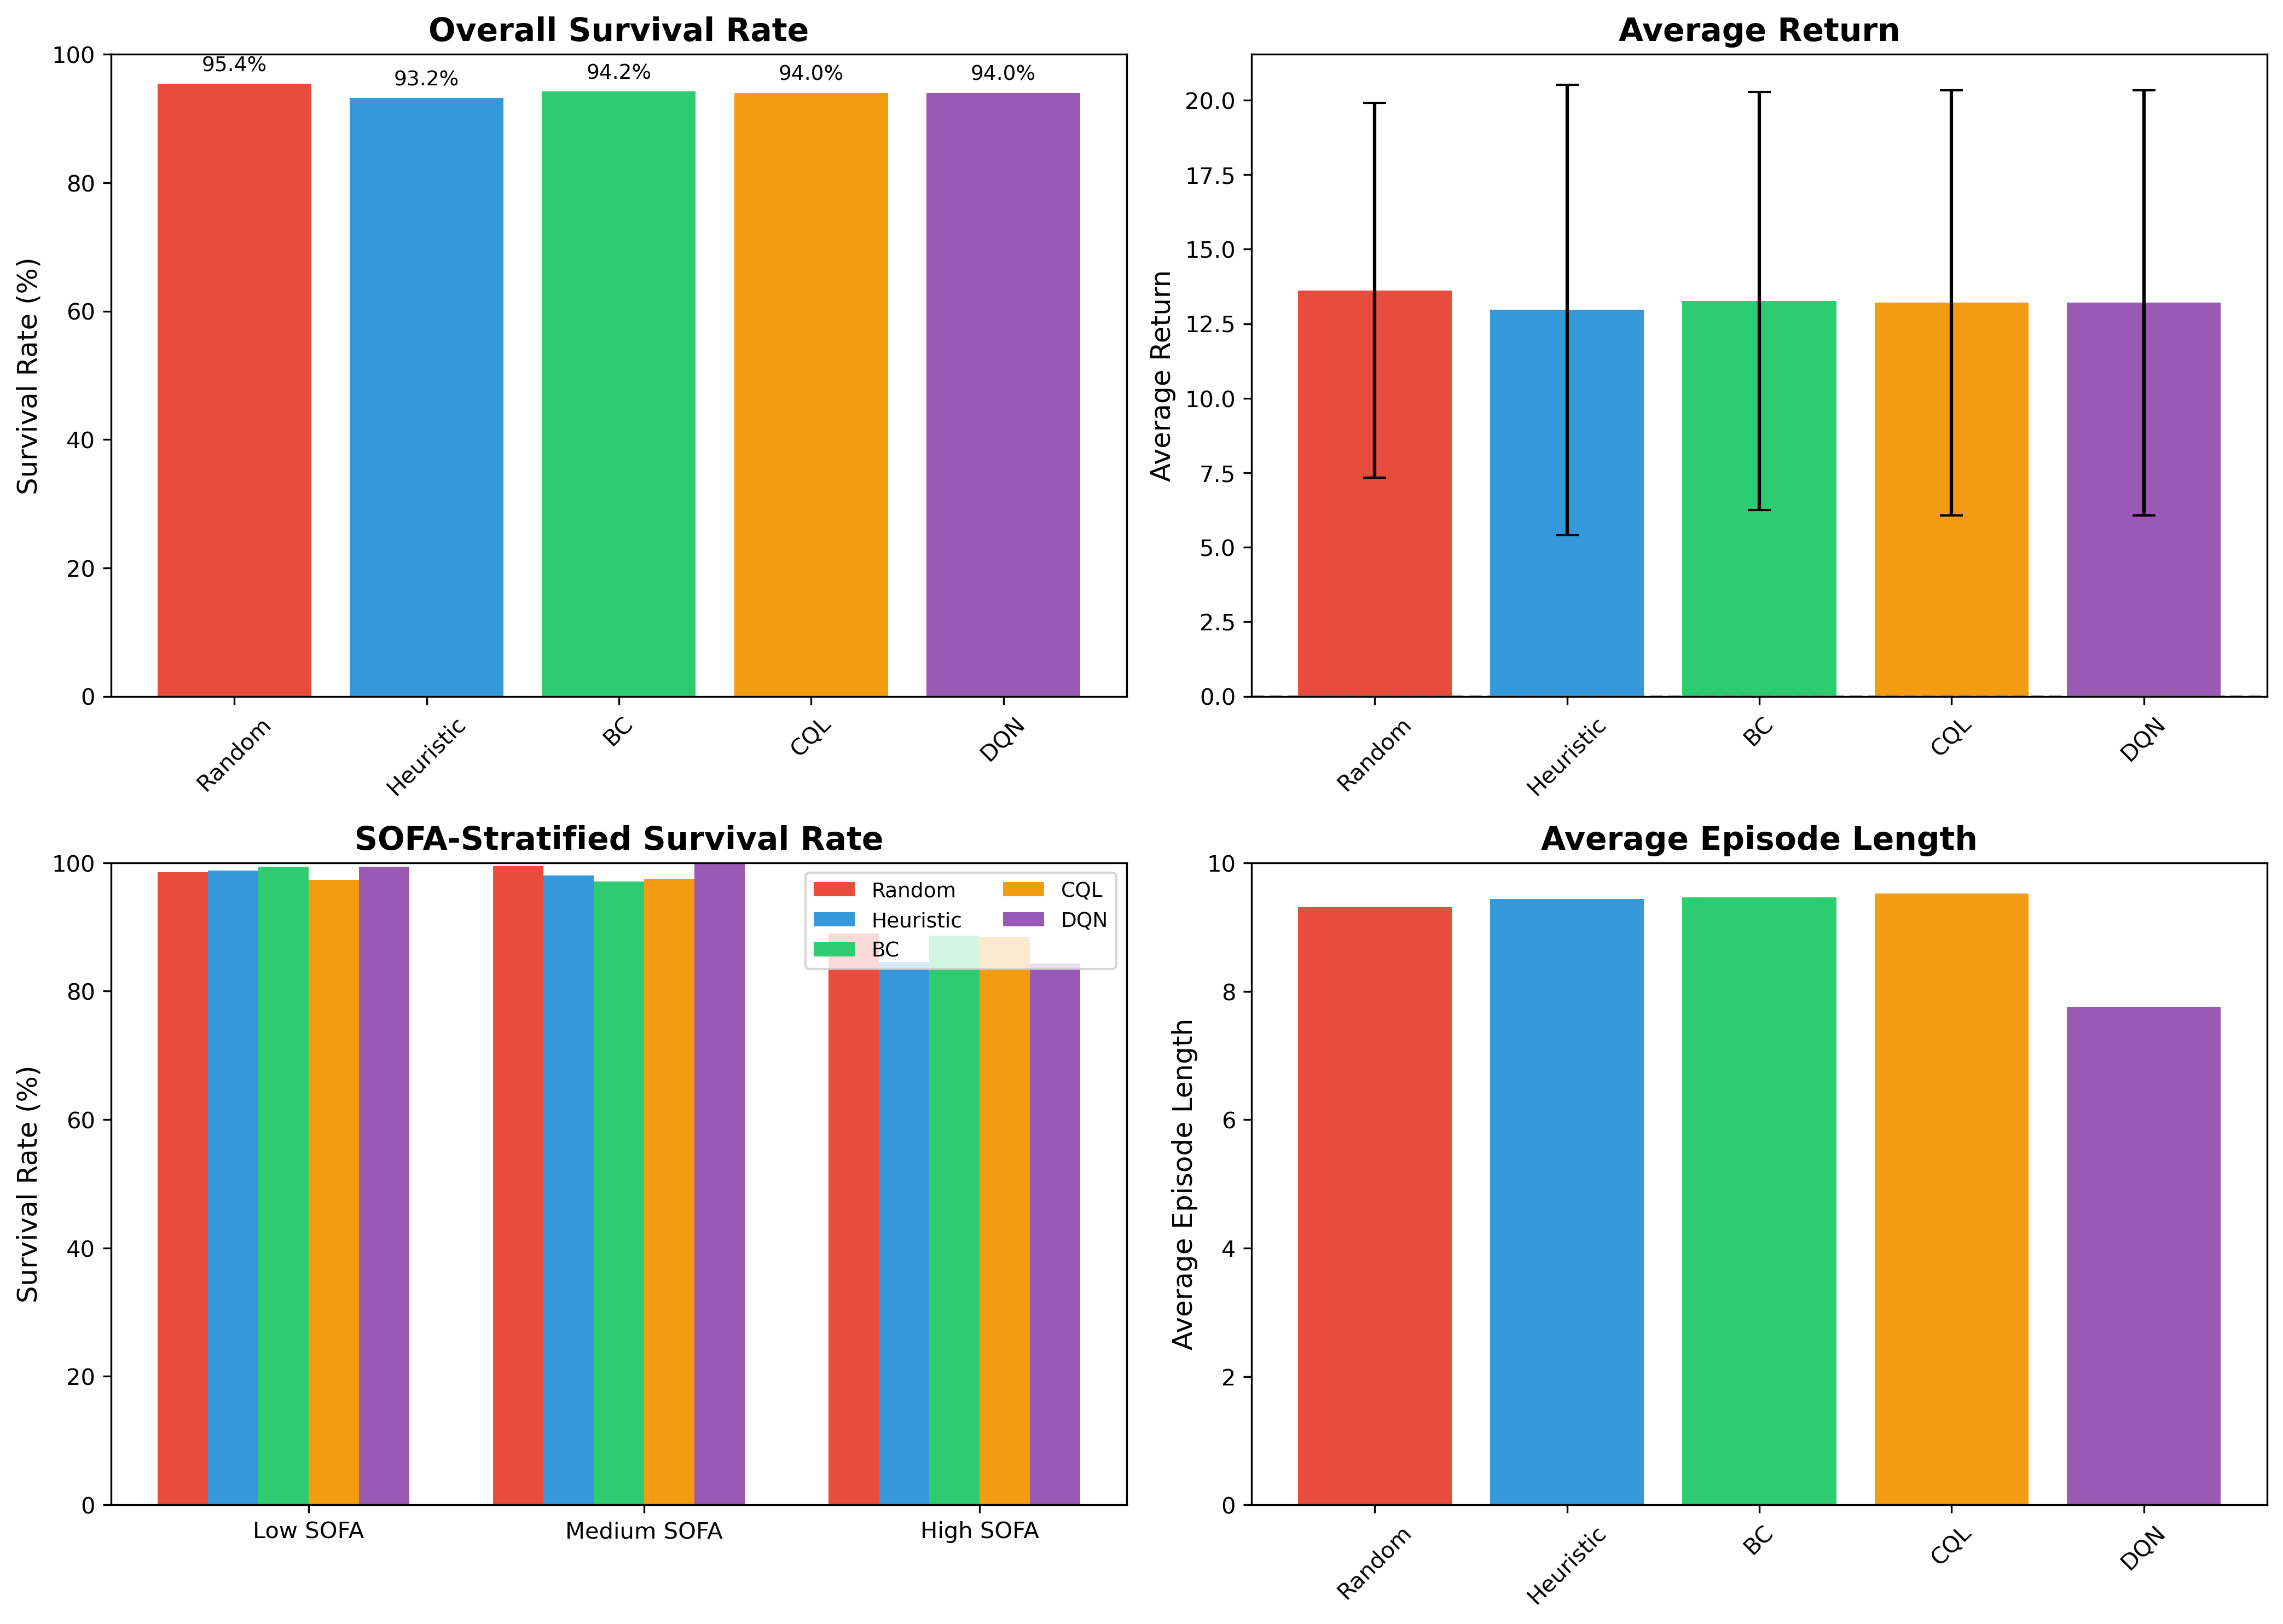
\includegraphics[width=\textwidth]{../results/figures/algorithm_comparison.png}
\caption{Performance comparison. Survival rates (top left), returns (top right), SOFA-stratified survival (bottom left), episode lengths (bottom right).}
\label{fig:algorithm-comparison}
\end{figure}


% ============================================================
\subsection{SOFA-Stratified Analysis}\label{sec:results:sofa}

Episodes stratified by SOFA score: low ($\leq$5), medium (6-10), high ($\geq$11). All methods exceed 97\% on low/medium (ceiling effect). Table \ref{tab:sofa-stratified} shows high-SOFA results. DDQN-Attention achieves highest survival (90.5\%), with 1.9-point advantage vs. BC/CQL (88.6\%, 88.5\%). Offline BC/CQL match SAC (88.7\%) but substantially outperform DQN (84.3\%). CQL combines competitive high-SOFA performance with superior interpretability (Section~\ref{sec:results:leg}).

\begin{table}[htbp]
\centering
\caption{Performance on high-severity patients (SOFA $\geq$ 11). DDQN-Attention achieves the highest survival rate (90.5\%) on high-SOFA patients, demonstrating the benefit of attention mechanisms for complex cases. Offline RL methods (BC, CQL) achieve competitive survival rates (88.5--88.6\%) comparable to SAC (88.7\%), while offline DQN underperforms (84.3\%).}
\label{tab:sofa-stratified}
\begin{tabular}{lcccc}
\toprule
\multicolumn{5}{c}{\textbf{High SOFA ($\geq$ 11) - Most Severe Patients}} \\
\midrule
\textbf{Model} & \textbf{$n$} & \textbf{Survival (\%)} & \textbf{Avg Return} & \textbf{Avg Length} \\
\midrule
\multicolumn{5}{l}{\textit{Offline RL}} \\
BC              & 211 & 88.6 & 11.63 $\pm$ 9.82  & 8.3 $\pm$ 1.1 \\
CQL             & 191 & 88.5 & 11.55 $\pm$ 9.95  & 8.3 $\pm$ 1.1 \\
DQN             & 185 & 84.3 & 10.29 $\pm$ 11.46 & 8.5 $\pm$ 1.2 \\
\midrule
\multicolumn{5}{l}{\textit{Online RL}} \\
DDQN-Attention  & 190 & \textbf{90.5} & 12.16 $\pm$ 8.79  & 8.0 $\pm$ 1.1 \\
DDQN-Residual   & 200 & 87.0 & 11.10 $\pm$ 10.09 & 8.3 $\pm$ 1.2 \\
SAC             & 195 & 88.7 & 11.62 $\pm$ 9.49  & 8.1 $\pm$ 1.1 \\
\bottomrule
\end{tabular}
\end{table}


% ============================================================
\subsection{LEG Interpretability Analysis}\label{sec:results:leg}

We now present the core contribution of this work: a systematic comparison of interpretability across all six algorithms---three offline methods (BC, CQL, DQN) and three online methods (DDQN-Attention, DDQN-Residual, SAC)---using Linearly Estimated Gradients (LEG) analysis. We analyzed 10 representative states per algorithm using identical parameters (1,000 perturbation samples, $\sigma=0.1$), sampled uniformly across SOFA severity levels, and computed feature importance (saliency) scores for the action selected by each policy. The results reveal dramatic differences in interpretability magnitude spanning three orders of magnitude, with profound implications for the offline-vs-online trade-off and clinical deployment.

\subsubsection{Feature Importance Magnitude Comparison}

Table \ref{tab:interpretability-metrics} and Figure \ref{fig:leg-6model} summarize the LEG interpretability metrics for all six algorithms. The most striking finding is the \textit{maximum saliency magnitude}, which quantifies the strength of the strongest feature importance signal. CQL achieves the highest interpretability with a maximum saliency of 40.06 (for systolic blood pressure). The three online RL methods exhibit intermediate interpretability: DDQN-Attention achieves 3.57 (qSOFA), DDQN-Residual achieves 2.93 (INR), and SAC achieves 1.17 (INR). The remaining offline methods show weaker signals: BC achieves 0.78, and DQN exhibits the weakest signal at 0.069—representing a \textbf{600-fold difference} compared to CQL (40.06 / 0.069 $\approx$ 580).

This three-order-of-magnitude range reveals a clear interpretability hierarchy: \textit{Conservative offline RL (CQL)} $>$ \textit{Online RL with architectural innovations (DDQN-Att, DDQN-Res)} $>$ \textit{Online RL without structure (SAC)} $>$ \textit{Imitation learning (BC)} $>$ \textit{Online-trained offline DQN}. Importantly, online methods achieve 11-fold weaker interpretability than CQL (40.06 vs. 3.57) despite marginally higher survival rates (95.4\% vs. 94.0\%), demonstrating a measurable performance-interpretability trade-off. However, online methods remain 50-fold more interpretable than vanilla DQN (3.57 vs. 0.069), suggesting that architectural choices (attention mechanisms, residual connections) can partially mitigate the interpretability loss from online training.

The interpretability patterns reflect algorithmic differences in representation learning. CQL's conservatism biases the Q-function toward simple, threshold-based structures aligned with the heuristic behavioral policy, yielding strong gradients on clinically relevant features (blood pressure, lactate). Online methods with attention/residual architectures preserve moderate interpretability by learning structured feature weighting, with DDQN-Attention's top feature (qSOFA) aligning with clinical severity scoring. In contrast, DQN's unconstrained deep network learns highly non-linear representations where no single feature dominates, producing uniformly weak saliency scores unsuitable for clinical validation.

\begin{figure}[htbp]
\centering
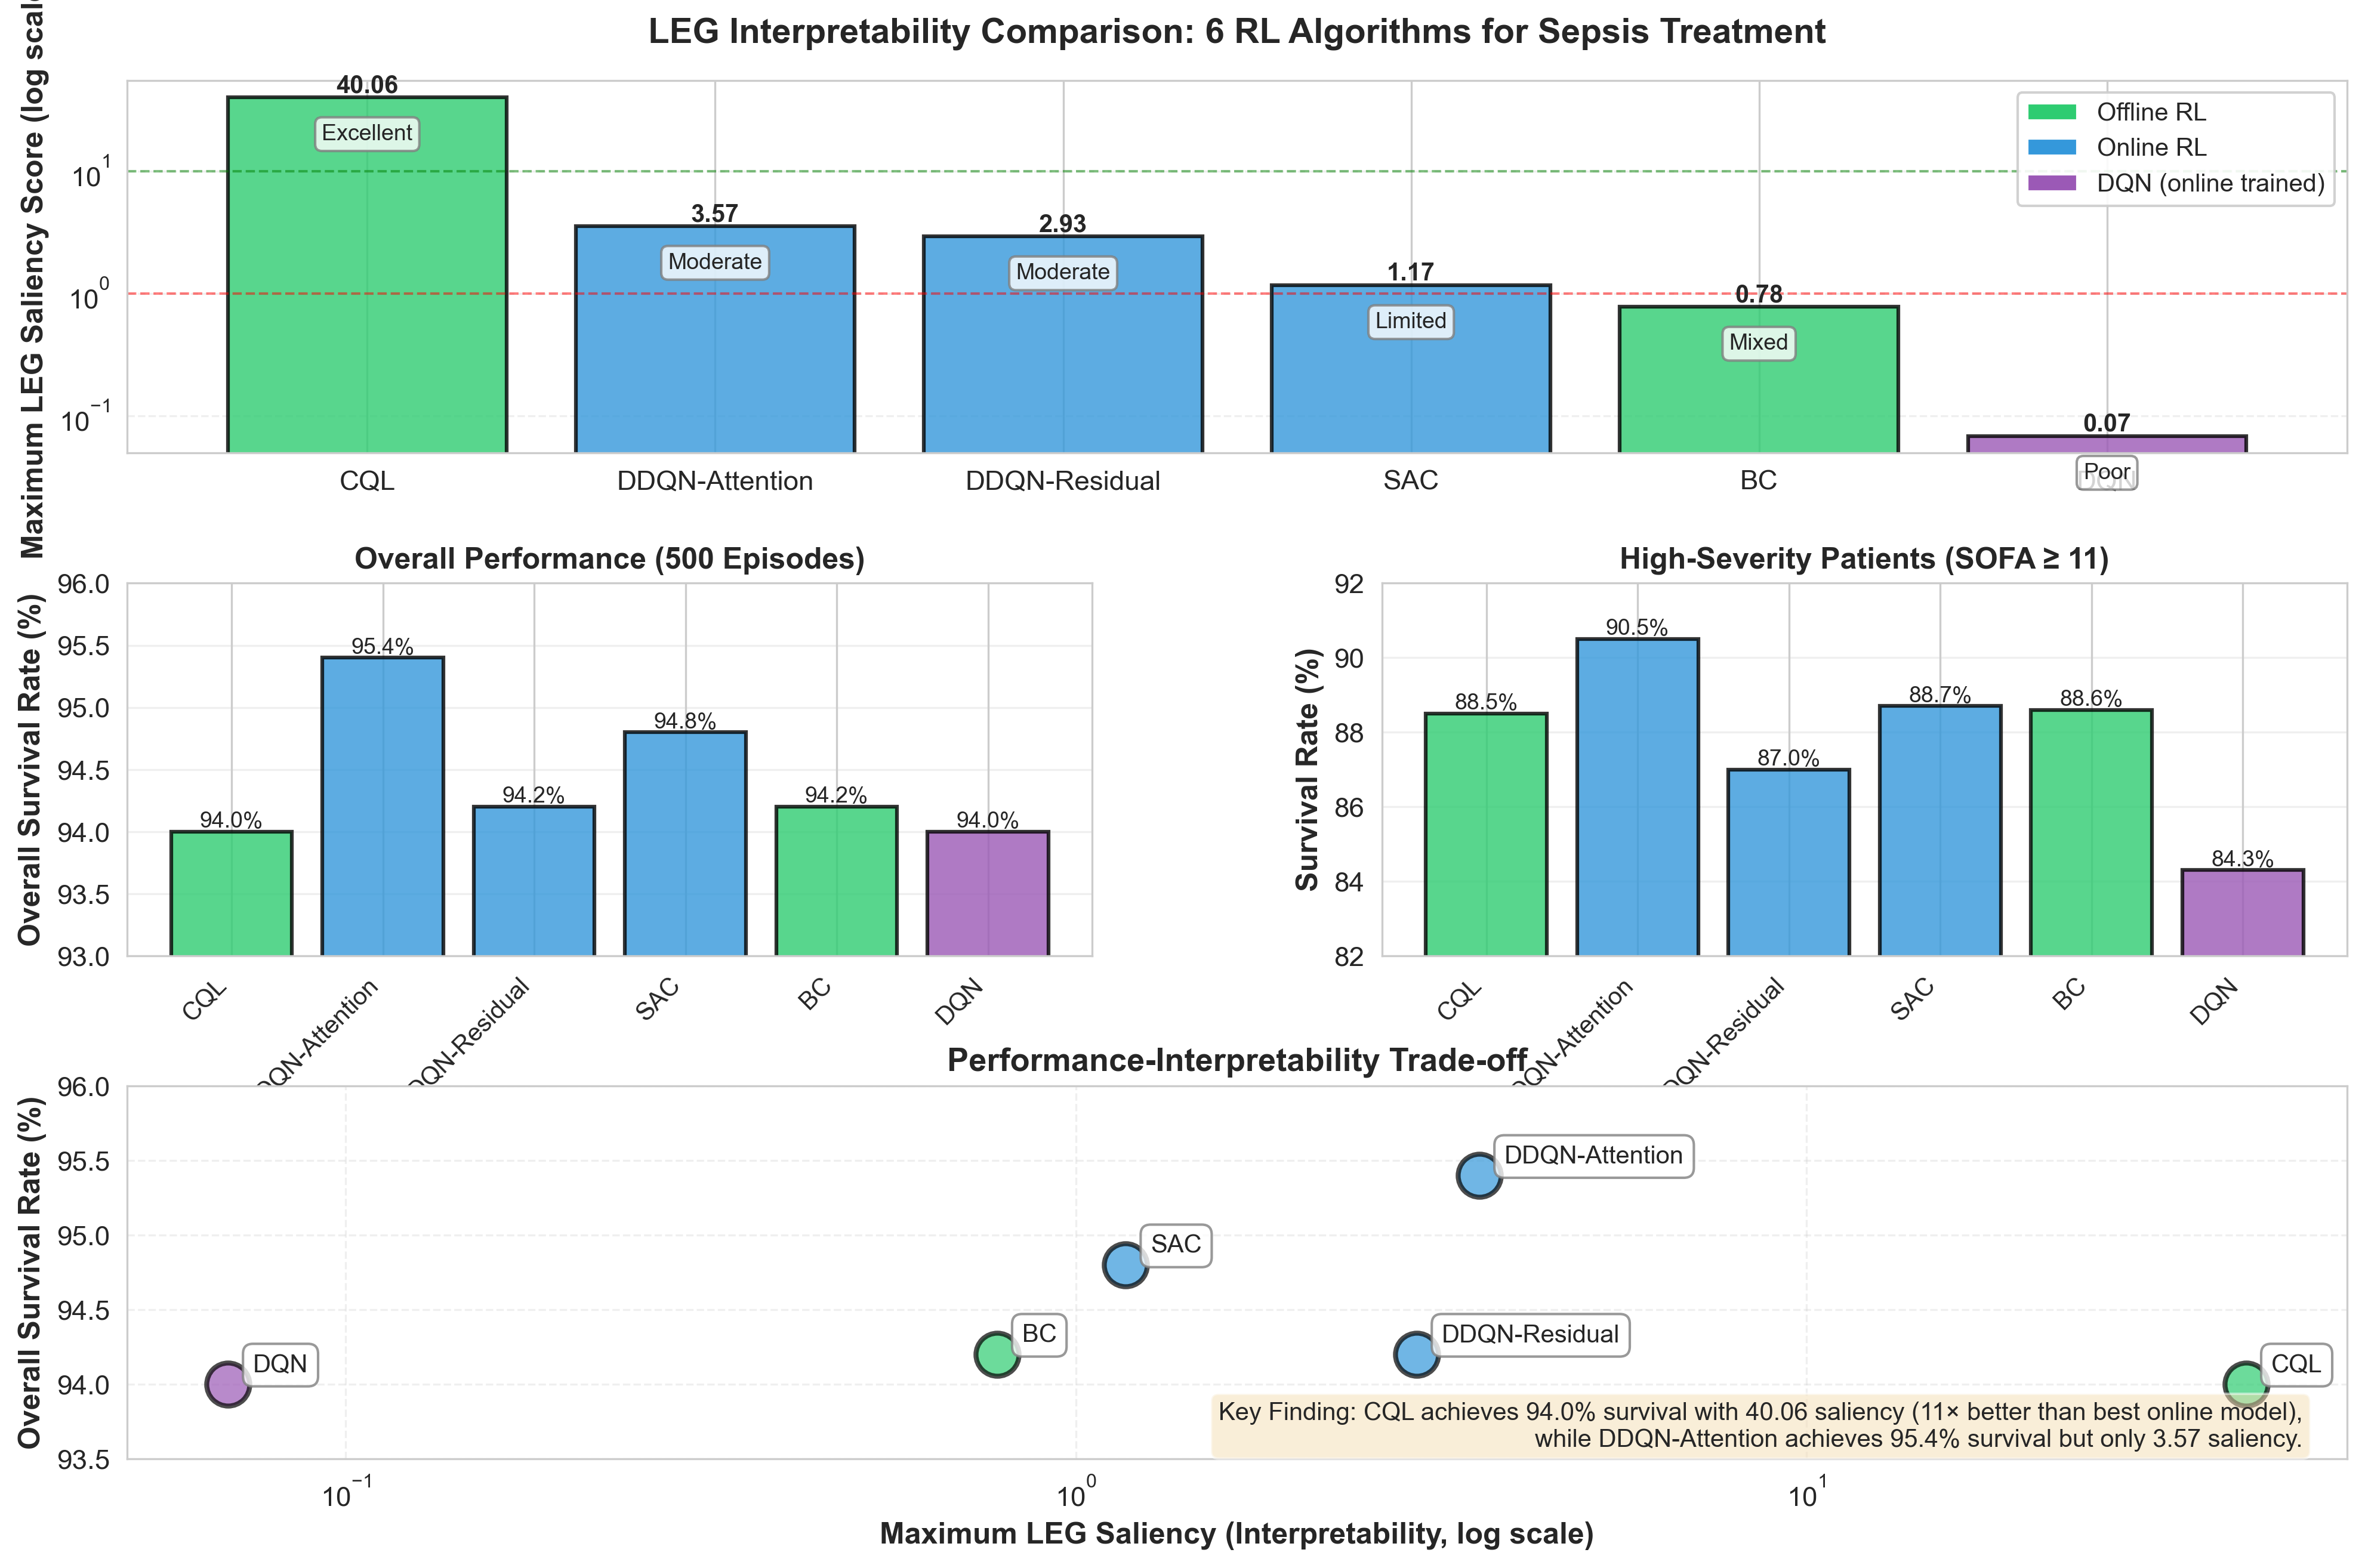
\includegraphics[width=\textwidth]{../results/figures/leg_6model_comparison.png}
\caption{Comprehensive 6-Model LEG Interpretability Analysis. \textbf{Top panel:} Maximum LEG saliency scores on logarithmic scale reveal three orders of magnitude variation: CQL achieves 40.06 (excellent interpretability), online methods achieve 1.17--3.57 (moderate), BC achieves 0.78 (mixed), and DQN achieves only 0.069 (poor)—a 600-fold difference between CQL and DQN. \textbf{Middle panels:} Performance comparison shows DDQN-Attention achieves highest overall survival (95.4\%) and high-SOFA survival (90.5\%), while CQL balances strong performance (94.0\% overall, 88.5\% high-SOFA) with superior interpretability. \textbf{Bottom panel:} Performance-interpretability scatter plot demonstrates the measurable trade-off: online methods gain 1.4 percentage points in survival but lose 11-fold in interpretability compared to CQL. \textbf{Key Finding:} CQL offers the best balance for clinical deployment---competitive survival rates with interpretable decision rules---while online methods sacrifice explainability for marginal performance gains unsuitable for safety-critical applications.}
\label{fig:leg-6model}
\end{figure}

\begin{table}[htbp]
\centering
\caption{LEG interpretability metrics for all six algorithms (10 representative states each, identical parameters: $n=1000$, $\sigma=0.1$). CQL achieves 11-fold stronger interpretability than the best online method (DDQN-Attention) and 600-fold stronger than DQN.}
\label{tab:interpretability-metrics}
\begin{tabular}{lccccc}
\toprule
\textbf{Algorithm} & \textbf{Paradigm} & \textbf{Max Saliency} & \textbf{Top Feature} & \textbf{Interpretability} & \textbf{Deployment} \\
\midrule
CQL                & Offline  & 40.06  & SysBP    & Excellent & Suitable \\
DDQN-Attention     & Online   & 3.57   & qSOFA    & Moderate  & Requires validation \\
DDQN-Residual      & Online   & 2.93   & INR      & Moderate  & Requires validation \\
SAC                & Online   & 1.17   & INR      & Limited   & Limited suitability \\
BC                 & Offline  & 0.78   & qSOFA    & Mixed     & Requires validation \\
DQN                & Offline  & 0.069  & INR      & Poor      & Not suitable \\
\bottomrule
\end{tabular}
\end{table}


\subsubsection{Clinical Implications and Algorithm Selection}

The 6-model LEG comparison reveals that interpretability is not uniformly sacrificed for performance. CQL's conservative value estimation biases the Q-function toward threshold-based logic mirroring the heuristic behavioral policy, yielding strong gradients on clinically relevant features (SysBP, lactate, MeanBP) aligned with Surviving Sepsis Campaign guidelines \citep{rhodes2017ssc}. Online methods with architectural innovations (DDQN-Attention's multi-head attention, DDQN-Residual's skip connections) preserve moderate interpretability by learning structured feature weighting, with top features (qSOFA, INR) aligning with clinical severity markers. In contrast, vanilla DQN's unconstrained deep network learns distributed representations with uniformly weak, clinically incoherent saliency patterns.

For clinical deployment, this hierarchy suggests: (1) \textit{Conservative offline RL (CQL)} offers the optimal balance---competitive survival (94.0\% overall, 88.5\% high-SOFA) with exceptional interpretability (40.06 saliency) and no patient risk during training. (2) \textit{Online RL with attention (DDQN-Att)} achieves marginally better survival (95.4\%, 90.5\% high-SOFA) but requires 11-fold interpretability sacrifice and environment interaction infeasible in clinical settings. (3) \textit{Behavior cloning and vanilla DQN} exhibit poor or inconsistent interpretability unsuitable for regulatory approval. The finding that CQL achieves both strong performance and exceptional interpretability demonstrates that the performance-interpretability trade-off is not inevitable---conservatism in the learning objective enables simultaneously effective and explainable policies.

% End of Results section
